\documentclass{beamer}
\usetheme{Madrid}

\usepackage[utf8]{inputenc}


\title[FGNs vs Adversarial Attacks] %optional
{Finite Gaussian Neurons}
\subtitle{A Defense Against Adversarial Attacks?}

\author[Felix Grezes] % (optional, for multiple authors)
{Felix Grezes}

\institute[CUNY GC] % (optional)
{
  \inst{}%
  Graduate Center\\
  City University of New York
}

\date[Thesis Proposal - Fall 2020] % (optional)
{Thesis Proposal Fall 2020}

\logo{
\includegraphics[height=1.5cm]{images/gc_logo_286_3_300px_511px.png}}

\begin{document}

\frame{\titlepage}

\begin{frame}
\frametitle{Table of Contents}
\tableofcontents
\end{frame}

%%%%  

\section{Abstract}

\begin{frame}
\frametitle{Abstract}
I introduce the Finite Gaussian Neuron, a novel neural network architecture.\\

My works aims to:
\begin{itemize}
    \item make it easy to convert existing models to the FGN architecture
    \item while preserving the existing model's behavior on real data
    \item and offering resistance against some adversarial attacks.
\end{itemize}

\end{frame}


\section{Introduction}

\begin{frame}{Introduction}
    
\end{frame}


\section{Related Work}

\begin{frame}{Related Work}
    
\end{frame}

\section{The Finite Gaussian Neuron}
\begin{frame}{The Classic Neuron}
% Classic neuron math
Neuron output: 
$$y = \varphi(l)$$
Linear component:
$$l=\sum_i x_i w_i$$

% classic neuron illustrated
\begin{center}
    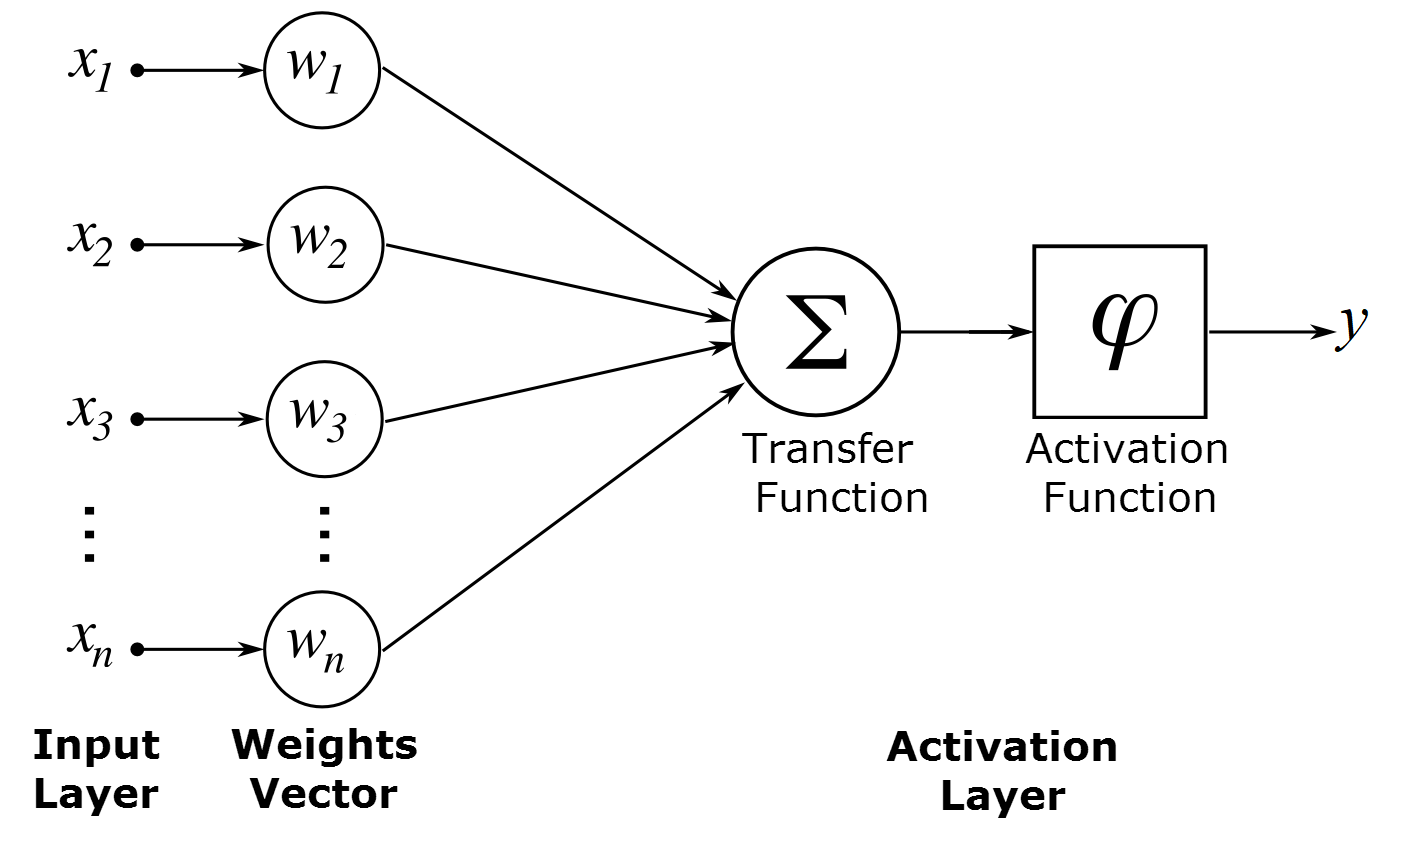
\includegraphics[width=0.75\textwidth]{images/artificial_neuron_model.png}
\end{center}
\end{frame}

\begin{frame}{The Finite Gaussian Neuron}
%%math
Neuron output:
$$ y = \varphi(\sum_i x_i w_i) * g$$ \\ 
Gaussian component:
$$ g = exp \left( \frac{-1}{\sigma^2}*\sum_{i}(x_i-c_i)^2 \right)$$
% $$ g = exp(\frac{-\sum_i (x_i-c_i)^2}{\sigma^2} )$$

%% gaussian component illustrated
\begin{center}
    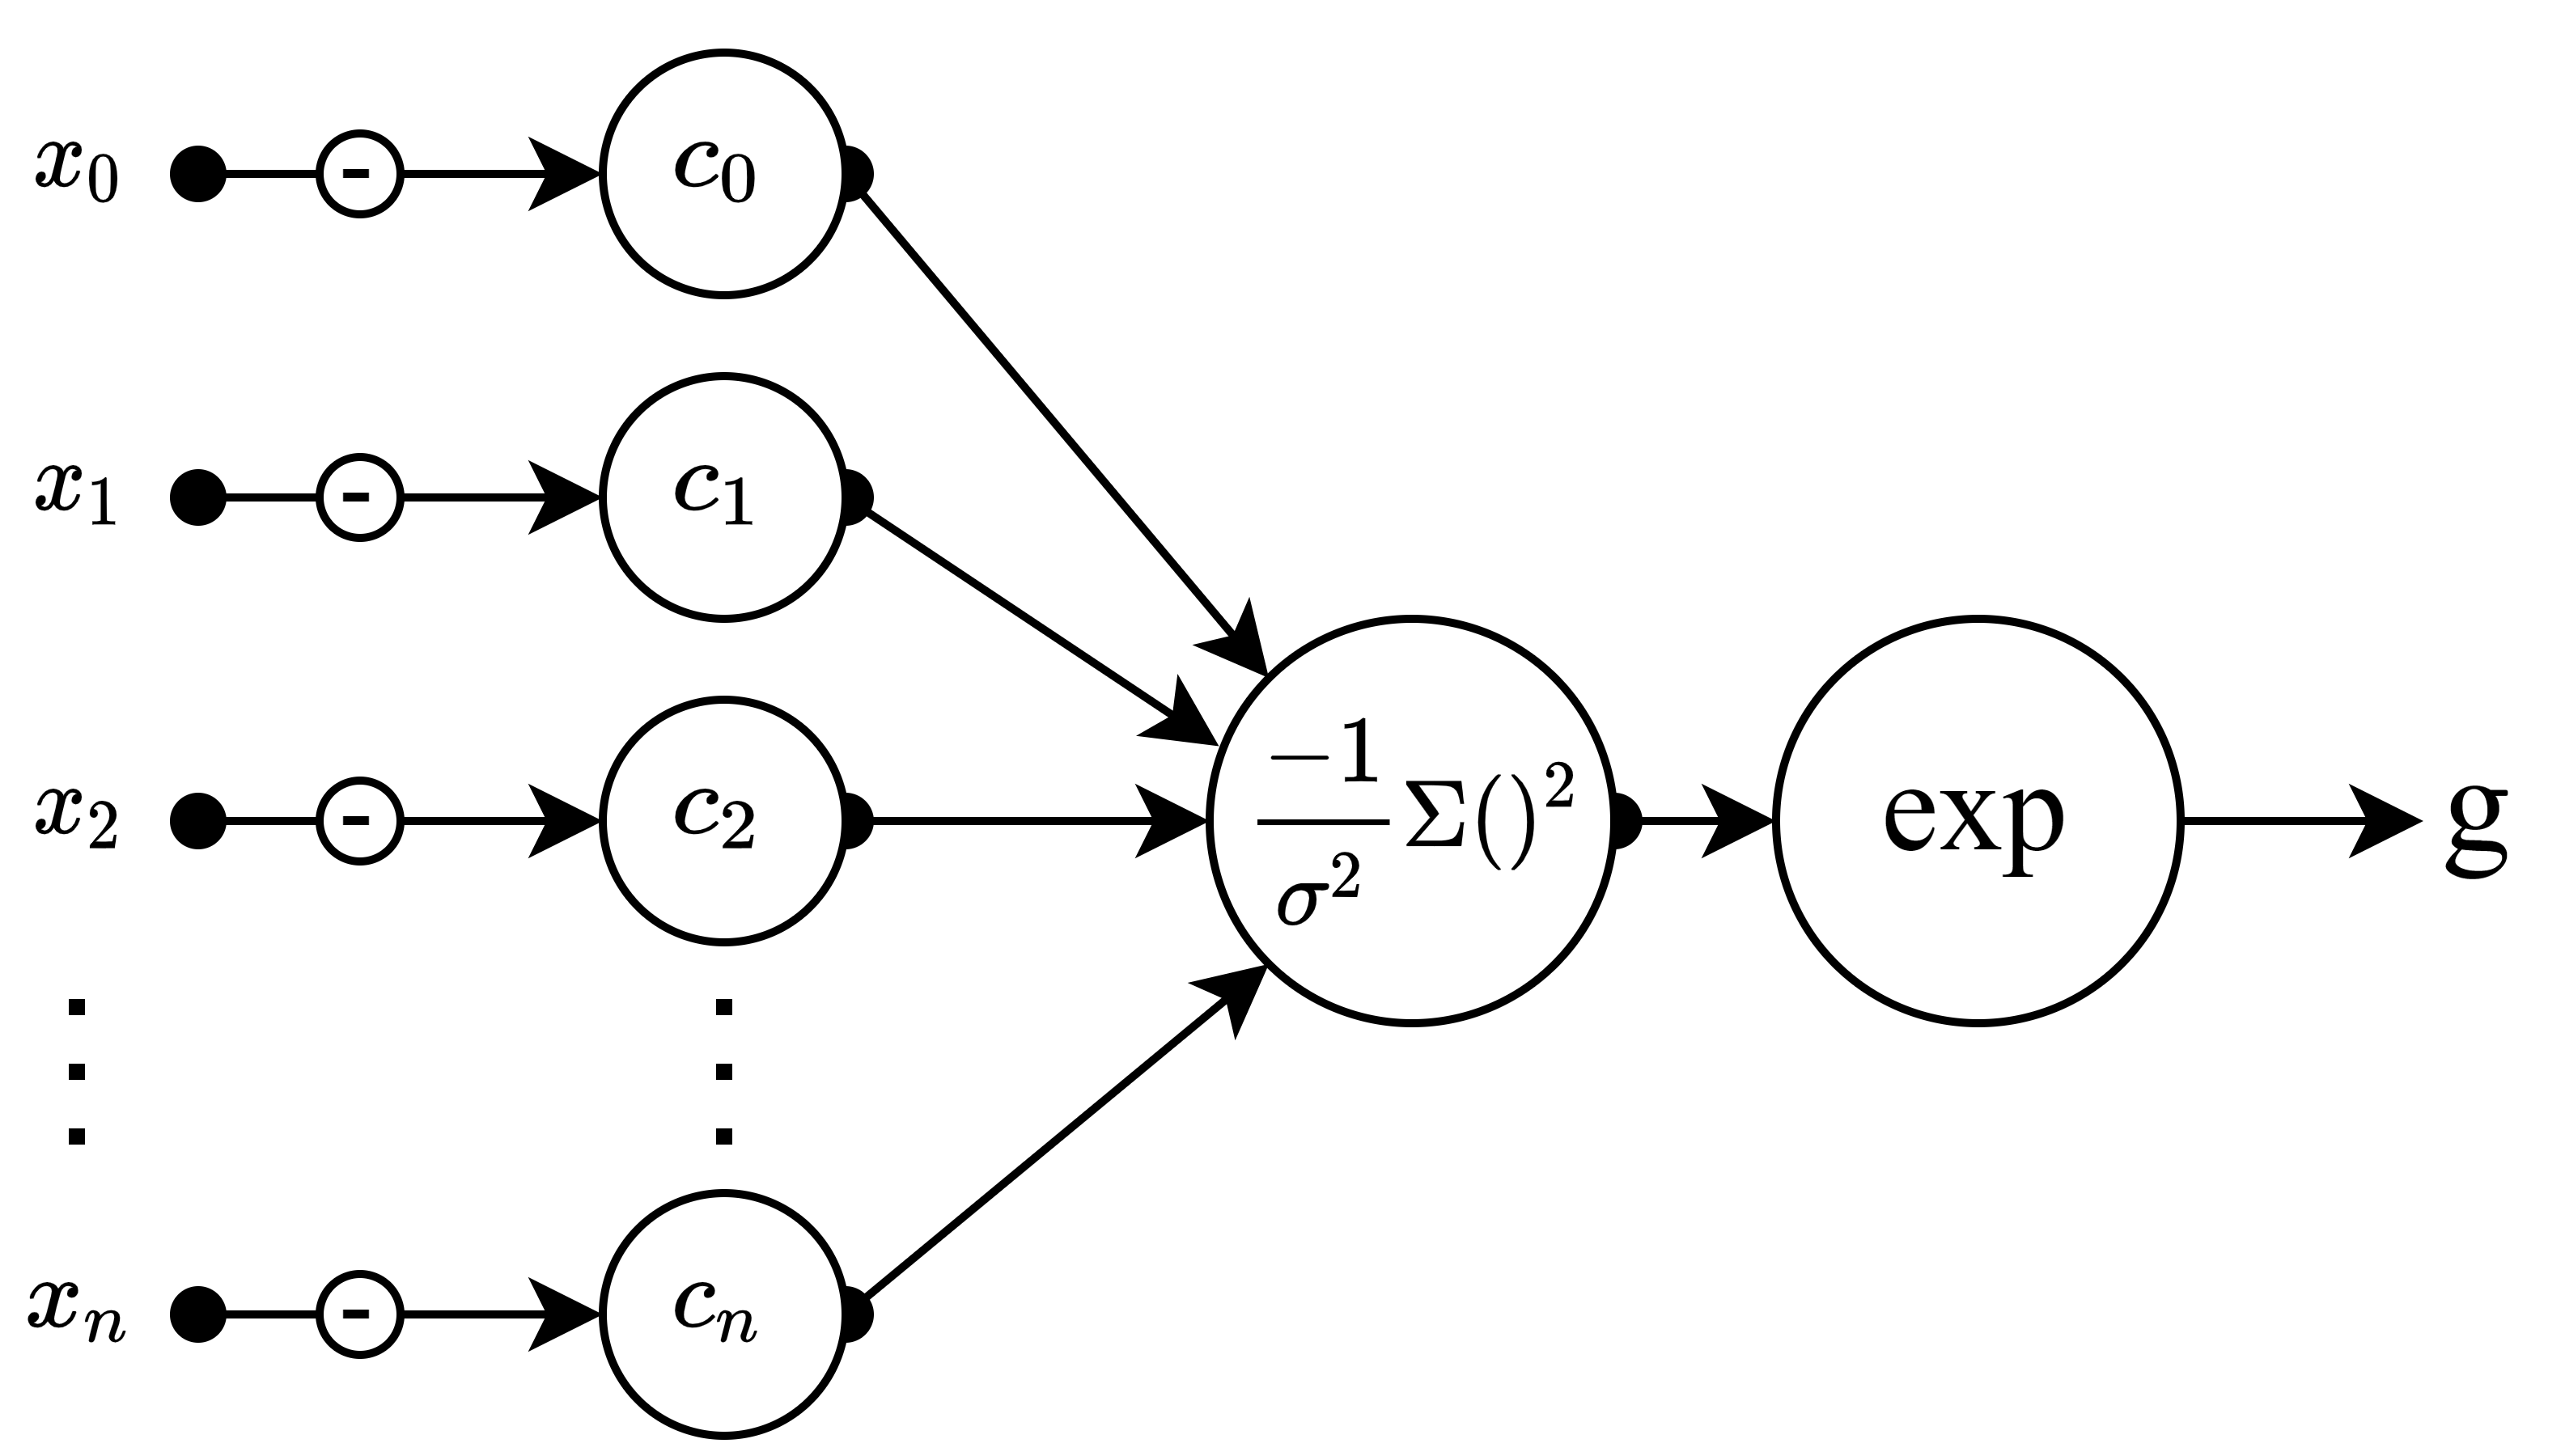
\includegraphics[width=0.5\textwidth]{images/fgn-gaussian-component.png}
\end{center}

\end{frame}

\begin{frame}{2D Illustration}
% 2 images for classic: linear and after non-linearity like tanh

% 2 images for fgn: gaussian component and combination 
\end{frame}




\end{document}